\chapter[DEICIDE]{DEICIDE:\\\LARGE A Framework for Distributional
  Reinforcement Learning of \Ito\ Diffusions}\label{c:deicide}

In the previous chapter, we derived an update rule for return measures
in which all return measures undergoing the update converge to a
unique fixed point, which satisfies the distributional HJB
equation \eqref{eq:dhjb}. In this chapter, we transform
this update rule to a concrete algorithm and demonstrate its
effectiveness against some benchmarks.

For the remainder of the thesis, we'll consider a
\hyperref[def:fd]{Feller-Dynkin process} $(\mathcal{X}, \mathcal{A},
\indexedabove{t}{P}, r, \gamma)$ for a finite (discrete) action space
$\mathcal{A}$ with respect to the probability space
$(\Omega, \mathcal{F}, \Pr)$ defined
\hyperref[def:probability-space]{previously} as well as the
\hyperref[def:canonical-filtration]{canonical filtration}
$\indexedabove{t}{\mathcal{F}}$. Moreover, we let assumptions
\ref{ass:method:density}, \ref{ass:method:c2}, and
\ref{ass:method:ito-diffusion} hold. Notably, assumption
\ref{ass:method:ito-diffusion} constrains the state process
$\indexedabove{t}{X}$ to the class of \Ito\ Diffusions; though by
\hyperref[thm:martingale-representation]{the Martingale Representation
  Theorem} this turns out to be quite robust. This chapter describes a
framework for designing distributional RL algorithms in this setting,
called \emph{\textbf{D}istributional \textbf{E}valuation of
\textbf{I}mplicitly-\textbf{C}ontrolled \textbf{I}tô \textbf{D}iffusion
\textbf{E}volutions}, or more compactly, DEICIDE.

Moving forward, we will derive tractable, convergent approximation algorithms
for continuous-time distributional RL in \S\ref{s:deicide:alg}. Given these
algorithms, we demonstrate their results on various benchmarks in
\S\ref{s:experiments}.


\section{Algorithms}\label{s:deicide:alg}
This section will give a description of DEICIDE algorithms for which
we provide numerical experiments in the sequel.

We will proceed as follows:
\begin{itemize}
  \item Based on the effects of spatial and statistical diffusivity due to
    imputation strategies as discussed in \S\ref{s:representation}, we will
    more concretely describe a tractable method of representing return
    distributions in \S\ref{s:deicide:alg:representation};
  \item In \S\ref{s:deicide:alg:learning}, we discuss how to compute unbiased
    gradient estimates in order to minimize the loss functional
    \eqref{eq:loss-functional} governing the policy evaluation gradient flow;
  \item We discuss strategies for exploration and optimal control in
    \S\ref{s:deicide:alg:optimal-control};
  \item Finally, based on the discussions of
    \S\ref{s:deicide:alg:representation}, \S\ref{s:deicide:alg:learning}, and
    \S\ref{s:deicide:alg:optimal-control}, in \S\ref{s:deicide:alg:algs} we
    present pseudocode for two concrete continuous-time distributional RL
    algorithms.
\end{itemize}

\subsection{Modeling the Return Measure
  Function}\label{s:deicide:alg:representation}
In order to approximate probability measures, we will employ
statistical functionals and imputation strategies as discussed in
\S\ref{s:representation}. More specifically, the gradient flow
optimization described by \eqref{eq:proximal-gradient} is
well-suited to ``particle approximations'' of probability measures --
that is, measures of the form

\begin{equation}
  \label{eq:deicide:particle-measure}
  \hat\returnmeasure(z\mid x) =
  \frac{1}{N}\sum_{i=1}^N\dirac{Z_i(x)}\qquad
  Z_i(x)\sim\returnmeasure(\cdot\mid x),\ i\in [N]
\end{equation}

The quantities being modeled are the Dirac locations $Z_i(x)$ in
\eqref{eq:deicide:particle-measure}, which notably can be interpreted as
samples from the target measure $\returnmeasure(\cdot\mid
x)$. Moreover, it is easy to verify that the quantiles of
$\hat\returnmeasure(z\mid x)$ are precisely the quantities $Z_i(x)$,
so we will simply approximate measures by their $\hat\tau_i$-quantiles
as statistical functionals, and the imputation strategy $\Phi$ given by

\begin{equation}
  \label{eq:deicide:imputation}
  \Phi(\indexedint{i}{N}{s}) = \frac{1}{N}\sum_{i=1}^N\dirac{s_i}
\end{equation}

While this representation is not Bellman-closed, it is approximately
Bellman-closed (so approximation error in TD-like updates decays to
$0$ as $N$ increases), it is simple to model, and it has demonstrated great
empirical success \citep{Dabney2018DistributionalRL}.

Concretely, in the tabular setting, this representation requires a
tensor of dimension $|\mathcal{X}||\mathcal{A}|N$. Thus, it requires
$N$ times the memory of a similar expected value RL algorithm. If we
venture into the world of function approximation, we represent the
statistical functionals by a set of function approximators
$\indexedint{i}{N}{Q^\theta}$, where $Q^\theta_i$ approximates
$\quantile{\returnmeasure(\cdot\mid x)}(\hat\tau_i)$ and $\theta$ is the
set of parameters. Implementing the function approximator with a
neural network that shares parameters among the quantile functions
until the final layer (a $N$-headed neural network), we again incur an
$N$-fold memory increase. 

\subsection{Learning Return Measures}\label{s:deicide:alg:learning}
As foreshadowed, the return measures are learned by optimizing
$\mathscr{F}_\beta$ as defined in \eqref{eq:proximal-gradient}. Recall
that the fixed point of this optimization only satisfies
\eqref{eq:shjb} in the limit as $\beta\to 0$. We treat $\beta$ as a hyperparameter.

Optimizing $\mathscr{F}_\beta$ via standard gradients is difficult,
however, for a couple of reasons.

\paragraph{Biased stochastic Wasserstein gradients}
As demonstrated by \citet{bellemare2017cramer}, estimating gradients
of the Wasserstein distances from samples are statistically biased
with high probability. Although \citet{Dabney2018DistributionalRL}
derives a method to minimize the $1$-Wasserstein distance in an
unbiased manner from samples, our optimization deals with the
$2$-Wasserstein distance.

\paragraph{Non-differentiability of the loss}
The entropy term $\mathcal{H}$ is not differentiable everywhere, so
gradients cannot blindly be computed. The Wasserstein Proximal
Gradient algorithm \citep{salim2020wasserstein} accounts for this with
a forward-backward Euler discretization scheme.

\paragraph{The irregularity of the approximated measures}
The measures we impute with $\Phi$ is by no means absolutely
continuous with respect to the Lebesgue measure. Additionally, we know
that the stationary solution of the gradient flow
\eqref{eq:loss-functional} is Gibbs measure with density proportional
to $e^{-\phi(\cdot)}$, which has no atoms. The imputed return measure
\emph{only} have atoms. Since \eqref{eq:loss-functional} can quickly
be reformulated as $\kl{\returnmeasure}{e^{-\phi}}$, the loss will
always be infinite. Fortunately, this problem has already been
accounted for as well. The Stein Variational Gradient Descent (SVGD)
algorithm \citep{liu2019stein} is able to circumvent this issue by
projecting the measure $\returnmeasure$ to a reproducing kernel
Hilbert space (RKHS) for the purpose of the update. Consequently the
algorithm is biased, as we likely don't know which RKHS, if any, the
return measure is part of. Alternatively, \citet{cuturi2013sinkhorn}
proposes the use of the \emph{Sinkhorn algorithm}
\citep{sinkhorn1967diagonal} to directly compute
$\mathscr{F}_\beta$. The Sinkhorn algorithm is itself an iterative
algorithm, which suggests that it may be slow when paired with an
iterative algorithm like SGD. However, \citet{cuturi2013sinkhorn}
shows that this algorithm happens to be quite fast, and
\citet{martin2020stochastically} employs this algorithm successfully
for the purpose of learning value distributions in discrete time.

In our experiments, we use the SVGD algorithm during the optimization
procedure, in a similar manner to \citet{Zhang2018PolicyOA}.

\subsection{Exploration and Optimal
  Control}\label{s:deicide:alg:optimal-control}
Due to the lack of theoretical guarantees surrounding return measure
convergence in the optimal control setting, we follow
\citet{Bellemare2017ADP, hessel2018rainbow} and perform the
optimization against policies with maximal means, as shown in
\S\ref{s:control}. For the purpose of exploration, which itself is a
highly complex problem, we stick to simple yet effective
$\epsilon$-greedy policies \citep{sutton2018reinforcement}:

\begin{equation}
  \label{eq:egreedy}
  \pi(a\mid x) =
  \begin{cases}
    \frac{1-\epsilon}{n^\star} + \frac{\epsilon}{|\mathcal{A}|} &
    a\in\arg\max_{a'\in\mathcal{A}}\Expect{\returnmeasure(\cdot\mid x,
      a')}\\
    \frac{\epsilon}{|\mathcal{A}|} & \text{otherwise}\\
  \end{cases}
\end{equation}

where

\begin{align*}
  n^\star =
  \left\lvert\arg\max_{a\in\mathcal{A}}\Expect{\returnmeasure(\cdot\mid
  x, a)}\right\rvert
\end{align*}

and $\epsilon\in(0,1]$.

\subsection{Quantile DEICIDE with Function
  Approximation}\label{s:deicide:alg:algs}
In this section, we provide pseudocode of algorithms based on DEICIDE
using quantiles as statistical functionals. The difference mainly are
due to the computation of the function $\mathscr{L}^\star$ as defined
in \eqref{eq:lstar}.

\paragraph{A model-based algorithm}
Algorithm \ref{alg:deicide:model-based} attempts to approximate
$\mathscr{L}^\star$ directly. In order to achieve this, we must learn
a stochastic model of the environment (a world model). Fortunately, we
have assumed that the state process is an \Ito\ diffusion, so we know
that $\Pr(X_{t+\delta}\mid X_t)$ is Gaussian-distributed for any
$\delta$. Our world model
$f_\pi^\psi:\mathcal{X}\times\mathcal{A}\to\probset{\mathcal{X}}$ with
parameters $\psi$ is implemented
as a neural network that outputs the location and
scale\footnote{Rather, we output the logarithm of the scale to ensure
  that the scale values are positive} parameters of a Gaussian
distribution. Additionally, to reduce complexity, we will assume the covariance
matrices of the stochastic dynamics are diagonal, so
$\pmb{\sigma}_\pi(x)\in\mathbf{R}^d$ will simply represent the diagonal of the
covariance matrix at state $x$. The network is trained to minimize $L^2$ error between
the samples from the world model and observed state differences, and
updates are computed by gradient descent via the reparameterization
trick \citep{kingma2013auto}. Then, since the quantile functions are
being approximated by differentiable function approximators, the
gradient and Hessian terms due to the
\hyperref[def:generator]{infinitesimal generator} of the \Ito\
Diffusion governing the state process can be computed, which can be
done without much trouble using an autodifferentation library such as
JAX \citep{jax2018github}.

\begin{algorithm}[h]
  \small
  \caption{Model-Based Q-DEICIDE}\label{alg:deicide:model-based}
  \begin{algorithmic}
    \For{each environment step $k$ and corresponding state transition
      $(x, a, r, x')$}
      \State{$\mathbf{Q}^\theta\leftarrow\mathbf{q}_{\returnmeasure(\cdot\mid
          x)}=\{\quantile{\returnmeasure(\cdot\mid
        x)}(\hat\tau_i) : i\in [N]\}$}; \Comment{Quantiles for return
        distribution at current state}
      \State{$\returnmeasure_k\leftarrow\Psi(\mathbf{Q^\theta})$};
      \State{$\hat{f}_\pi\leftarrow\delta^{-1}(x' - x)$};
      \Comment{Dynamics estimate}
      \State{$(f_\pi, \log\pmb{\sigma}_\pi)\leftarrow
        f_\pi^\psi(x, a)$};
      \State{$\tilde{f}_\pi^\psi\leftarrow F\sim\mathcal{N}(f_\pi,
        \pmb{\sigma}_\pi)$};\Comment{Sample from world model}
      \State{$\mathcal{L}_f(\psi)\leftarrow \frac{1}{2}(\hat{f}_\pi -
        \tilde{f}_\pi^\psi)^2$}; 
      \State{$\psi\leftarrow\psi -
        \alpha_\psi\nabla_\psi\mathcal{L}_f(\psi)$}; 
      \Comment{Gradient computed by reparameterization trick} 
      \For{$i\in\{1,\dots,N\}$}
        \State{$\mathscr{H}(q_i)\leftarrow r + q_i\log\gamma +
          \langle\nabla_x\quantile{\returnmeasure(\cdot\mid
            x)}(\hat\tau_i),f_\pi\rangle$}; 
        \State{$\psi(q_i)\leftarrow
          \frac{1}{2}\left(\mathscr{H}(q_i) +
            \frac{1}{2}\quadraticform{\pmb{\sigma}_\pi}{\hessian{x}\quantile{\returnmeasure(\cdot\mid
                x)}(\hat\tau_i)}\right)^2$};
      \EndFor
      \State{$\widetilde{\varrho}\leftarrow
        e^{-\phi(\cdot)}$};\Comment{Unnormalized target distribution}
      \State{$\widehat{\mathbf{Q}^\theta}\leftarrow \mathbf{Q}^\theta -
        \delta\mathsf{SVGD}_{\theta}(\kl{\returnmeasure_k}{\widetilde\varrho},\kappa)$};\Comment{WGF
        KL step with kernel $\kappa$ \citep{liu2019stein}} 
      \State{$\theta\leftarrow\theta -
        \nabla_\theta\wassermetric^2(\Psi(\widehat{\mathbf{Q}^\theta}),
        \returnmeasure(\cdot\mid x))$};\Comment{WGF $2$-Wasserstein trust region
        step \citep{Zhang2018PolicyOA}}
    \EndFor
  \end{algorithmic}
\end{algorithm}

An issue with this implementation is that optimization tends to be
unstable. Note that Algorithm \ref{alg:deicide:model-based} is not
actually a temporal difference learning algorithm, since the
``difference'' is measured instantaneously. Consequently, there is
no clear separation between the quantile function and a target
function of some sort, which prohibits the use of semi-gradient
updates that have are ubiquitous in the RL literature \citep{sutton2018reinforcement}.

\paragraph{A finite differences algorithm}
We also consider a model that is more stable under differential
optimization methods. Rather than computing the actual gradient and
Hessian of the quantile functions, we may employ a \emph{finite
  differences} scheme to approximate these computations. Since the
characterization of each quantile function of the return distribution
\eqref{eq:shjb} has precisely the same structure as the HJB
equation, we apply a finite differences computation
proposed by \citet{Munos2004ASO}. A byproduct of this scheme is that
we now get to compute updates based on temporal differences, allowing
us to stabilize the updates by computing semi-gradients. This is shown
in Algorithm \ref{alg:deicide:fd}.

\begin{algorithm}[h]
  \small
  \caption{Model-Based Q-DEICIDE with Finite Differences}\label{alg:deicide:fd}
  \begin{algorithmic}
    \For{each environment step $k$ and corresponding state transition
      $(x, a, r, x')$}
      \State{$\mathbf{Q}^\theta\leftarrow\mathbf{q}_{\returnmeasure(\cdot\mid
          x)}=\{\quantile{\returnmeasure(\cdot\mid
        x)}(\hat\tau_i) : i\in [N]\}$}; \Comment{Quantiles for return
        distribution at current state}
      \State{$\returnmeasure_k\leftarrow\Psi(\mathbf{Q^\theta})$};
      \State{$\hat{f}_\pi\leftarrow\delta^{-1}(x' - x)$};
      \Comment{Dynamics estimate}
      \State{$(f_\pi, \log\pmb{\sigma}_\pi)\leftarrow
        f_\pi^\psi(x, a)$};
      \State{$\tilde{f}_\pi^\psi\leftarrow F\sim\mathcal{N}(f_\pi,
        \pmb{\sigma}_\pi)$};\Comment{Sample from world model}
      \State{$\mathcal{L}_f(\psi)\leftarrow \frac{1}{2}(\hat{f}_\pi -
        \tilde{f}_\pi^\psi)^2$}; 
      \State{$\psi\leftarrow\psi -
        \alpha_\psi\nabla_\psi\mathcal{L}_f(\psi)$}; 
      \Comment{Gradient computed by reparameterization trick} 
      \For{$i\in\{1,\dots,N\}$}
      \State{$h\leftarrow\frac{1}{\epsilon^2}\bot\left(\pmb{\sigma}_\pi^\bot\left[q_i^\theta(x
          + 2\epsilon\pmb{\sigma}_\pi) - 2q_i^\theta(x +
          \epsilon\pmb{\sigma}_\pi) + q_i^\theta\right]\right)$};
      \State{$\phi(q_i)\leftarrow\frac{1}{2}(\delta r +
        \gamma^\delta\bot(q_i^\theta(x')) + \frac{\delta}{2}h - q_i^\theta(x))^2$};
      \EndFor
      \State{$\widetilde{\varrho}\leftarrow
        e^{-\phi(\cdot)}$};\Comment{Unnormalized target distribution}
      \State{$\widehat{\mathbf{Q}^\theta}\leftarrow \mathbf{Q}^\theta -
        \delta\mathsf{SVGD}_{\theta}(\kl{\returnmeasure_k}{\widetilde\varrho},\kappa)$};\Comment{WGF
        KL step with kernel $\kappa$ \citep{liu2019stein}} 
      \State{$\theta\leftarrow\theta -
        \nabla_\theta\wassermetric^2(\Psi(\widehat{\mathbf{Q}^\theta}),
        \returnmeasure(\cdot\mid x))$};\Comment{WGF $2$-Wasserstein trust region
        step \citep{Zhang2018PolicyOA}}
    \EndFor
  \end{algorithmic}
\end{algorithm}

\section{Experiments}\label{s:experiments}
\subsection{A Stochastic Extension of Munos' Toy Problem}
We begin by testing DEICIDE in a very simple environment, which is a
slight modification of the toy example presented by
\citet{Munos2004ASO}. The task consists of controlling a particle on
$\mathcal{X} = [0,1]$ with actions in $\mathcal{A} = \{-1, 1\}$. The
dynamics are simply $\frac{dx}{dt} = f(x, a) = a$. The reward signal
is zero in the interior of $\mathcal{X}$. When the particle reaches a
boundary, the episode ends and the agent is given a stochastic reward
sampled from a distribution corresponding to the endpoint it
reached. Specifically,

\begin{align*}
  r(1) &\sim \mathcal{N}(2, 2)\\
  r(0) &\sim \mathcal{N}(1, 1)\\
\end{align*}

We are interested in observing how existing distributional RL
algorithms perform in this environment, and if our DEICIDE algorithms
perform more favorably.

As an overview, we present a bird's eye view of the return
distribution function learned by both the discrete-time and
continuous-time algorithms.

\begin{figure}[h]
  \newcommand{\munosbirdscale}{0.275}
  \centering
  \begin{minipage}{0.49\linewidth}
    \centering
    \textsc{Quantile Regression TD}\\
    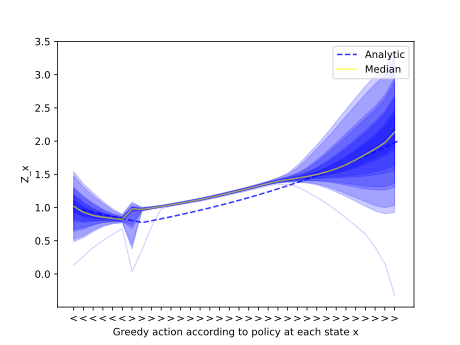
\includegraphics[scale=\munosbirdscale]{results/dt51-munos-overview}
  \end{minipage}%
  \begin{minipage}{0.49\linewidth}
    \centering
    \textsc{DEICIDE TD}\\
    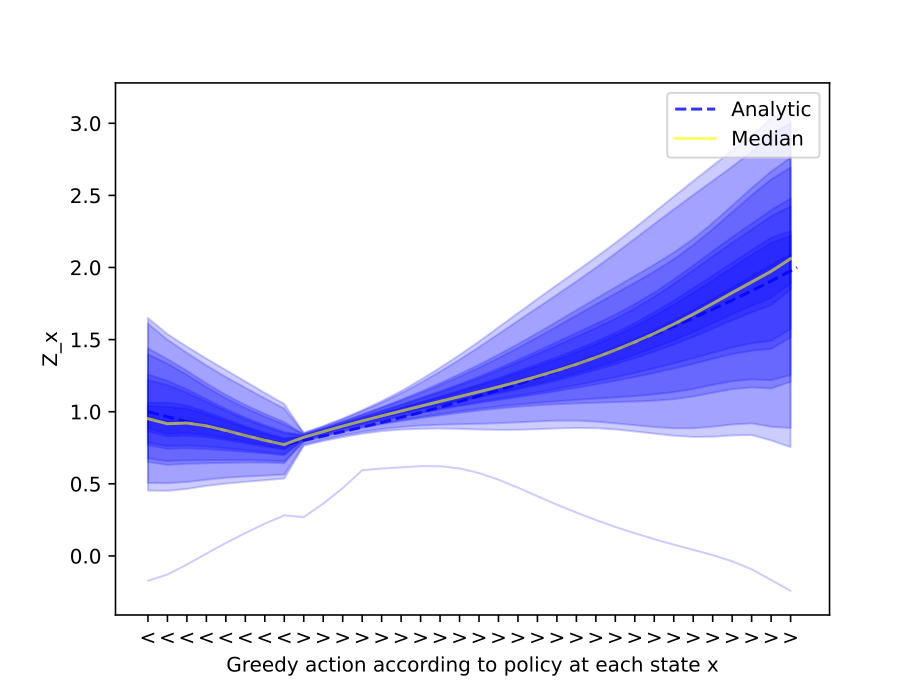
\includegraphics[scale=\munosbirdscale]{results/ct51-munos-overview}
  \end{minipage}%
  \caption{Bird's eye view of the learned return distribution
    functions}
  \label{fig:exp:munos:bird}
\end{figure}

As in the expected value RL case, we see that the median of the return
measure functions converges nicely to the ground truth in our
continuous-time algorithm, however the discrete-time algorithm is
disturbed at the point of non-differentiability. More interestingly,
the return measure function learned in the discrete-time algorithm has
some bizarre properties:
\begin{itemize}
\item The distributions are not symmetric. Since the agent only
  receives a single reward which is Gaussian-distributed, we should
  expect the return measures to be Gaussian, especially near the
  endpoints. This is not the case at all for the discrete-time
  algorithm.
\item The variance of the return measure vanishes very rapidly as
  the state moves away from the boundaries, to the point where the
  return measures are effectively deterministic in most of the state
  space. This is not the case with our continuous-time algorithm.
\item Aside from the return measures \emph{and} their medians being
  off, the the return measures also do not induce an optimal policy in
  our experiment.
\end{itemize}

We can examine some of these oddities further. Comparing the return
measures estimated near the endpoints, we observe the data shown in
Figure \ref{fig:exp:munos:bounds}.

\begin{figure}[h]
  \centering
  \newcommand{\munosscanscaledt}{0.73}
  \newcommand{\munosscanscalect}{0.73}
  \textsc{Quantile Regression TD}\\
  \begin{minipage}[t]{0.495\linewidth}
    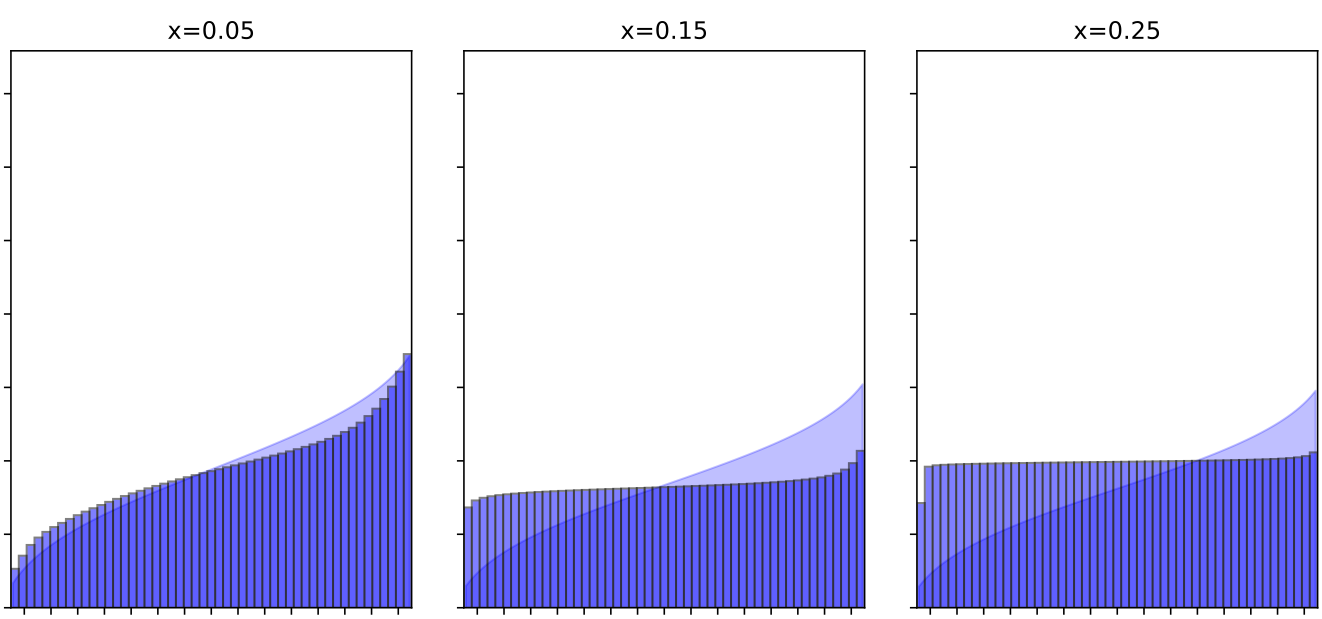
\includegraphics[scale=\munosscanscaledt]{results/dt51-munos-scan-left}
  \end{minipage}%
  \begin{minipage}[t]{0.495\linewidth}
    \centering
    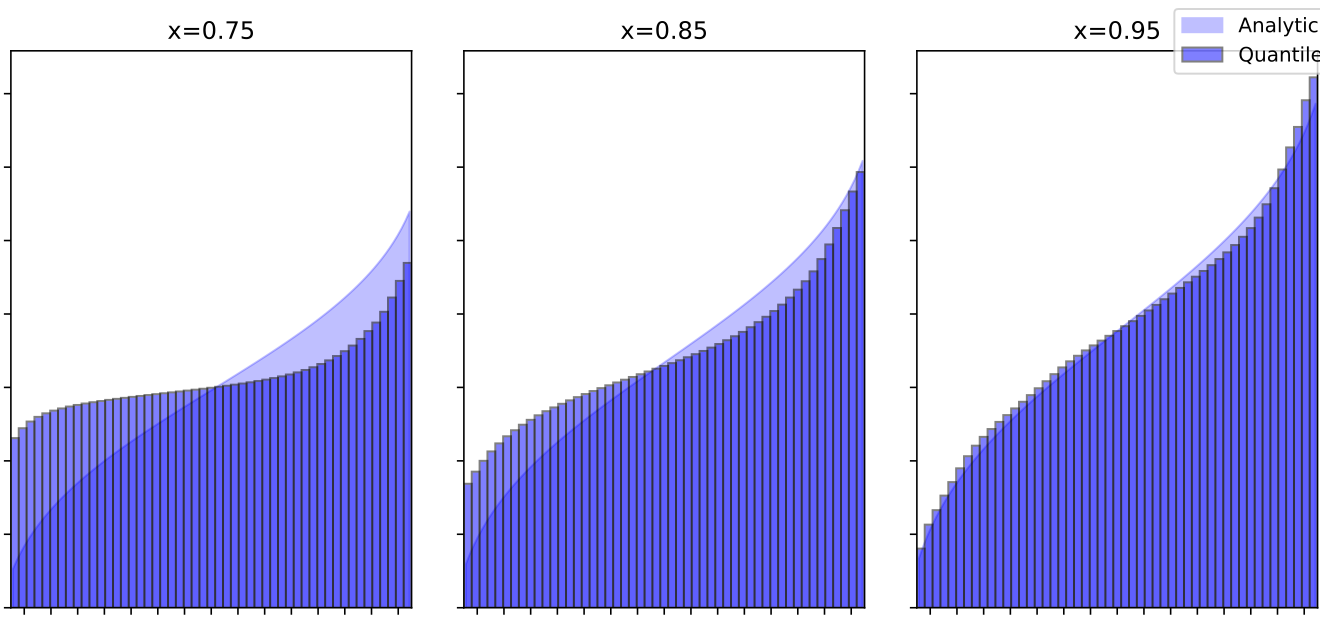
\includegraphics[scale=\munosscanscaledt]{results/dt51-munos-scan-right}
  \end{minipage}
  \textsc{DEICIDE TD}\\
  \begin{minipage}[t]{0.495\linewidth}
    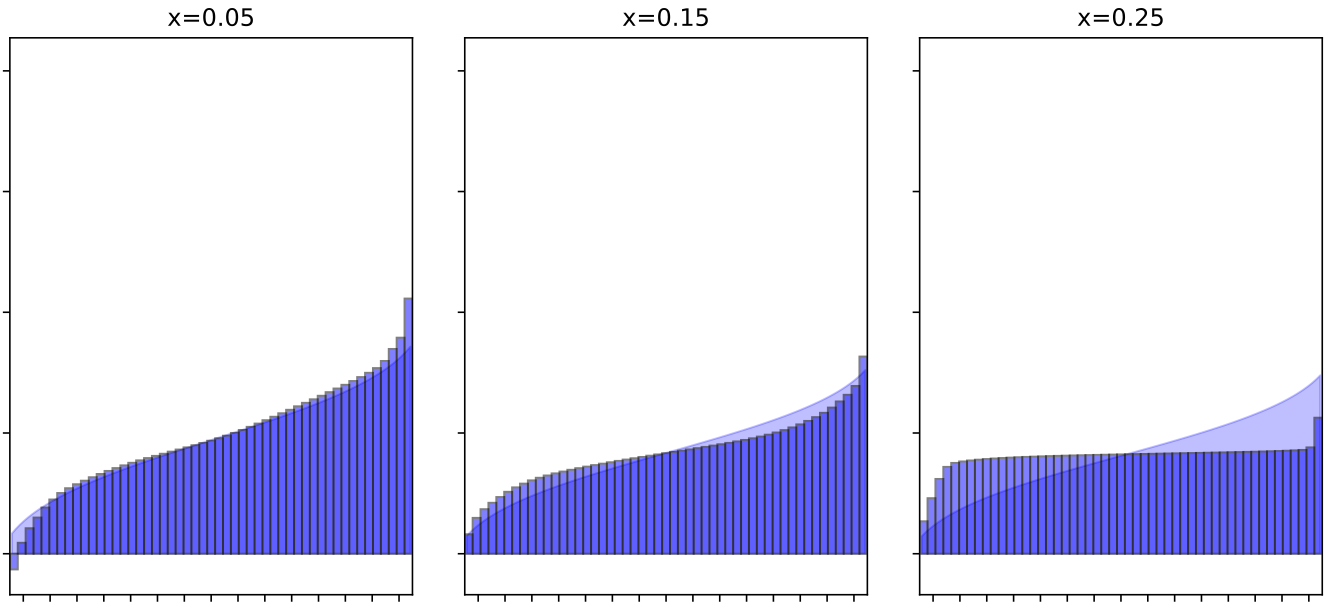
\includegraphics[scale=\munosscanscalect]{results/ct51-munos-scan-left}
  \end{minipage}%
  \begin{minipage}[t]{0.495\linewidth}
    \centering
    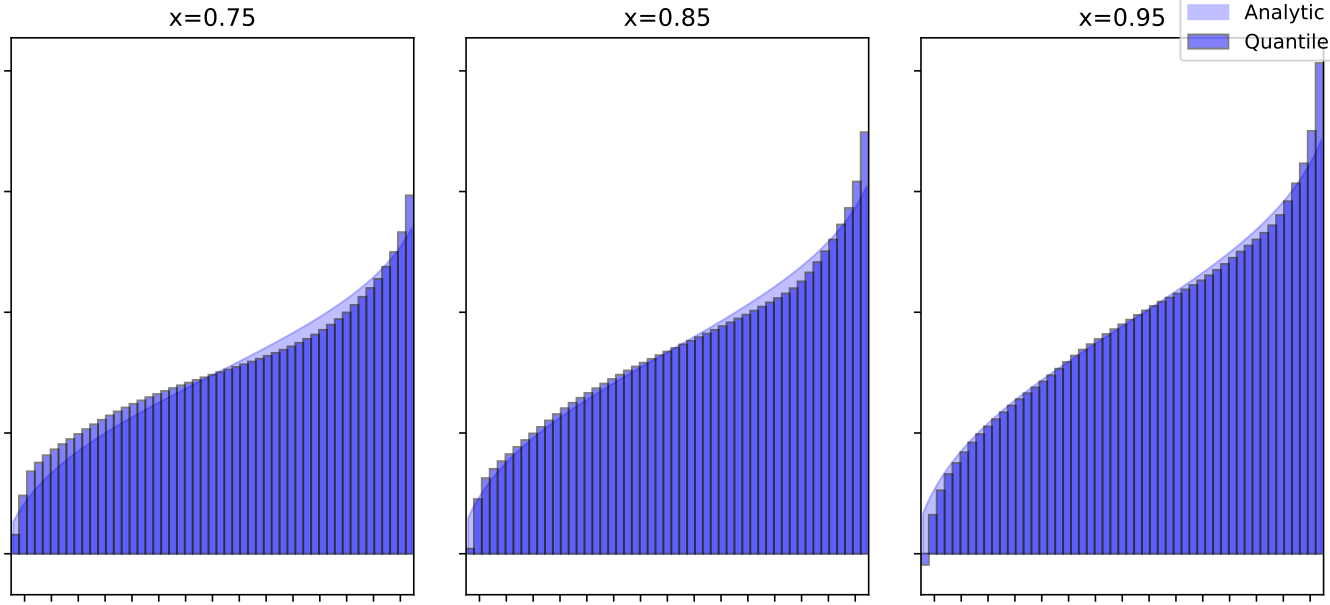
\includegraphics[scale=\munosscanscalect]{results/ct51-munos-scan-right}
  \end{minipage}
  \caption[Estimates of the return measures near the boundaries]{%
    Quantile functions learned by both algorithms near the
    boundaries. The horizontal axis is the quantile $\tau$ and the
    vertical axis is the $\tau$-quantile. The pale shaded region is
    the ground truth quantile function. The state input is indicated
    above each graph.
  }
  \label{fig:exp:munos:bounds}
\end{figure}

We see that both algorithms tend to shed variance in the interior of
the state space, however DEICIDE tends to model the full distribution
substantially better, as we expect from Figure \ref{fig:exp:munos:bird}.

\subsection{Deterministic Environments}
Recall that the analysis we presented for return distributions always
assumed that the return measures are absolutely continuous with
respect to the Lebesgue measure. A reasonable question to ask, then,
is how DEICIDE algorithms behave in deterministic environments where
the true returns have distributions $\dirac{V^\pi(\cdot)}$, since
these distributions most certainly do not satisfy this assumption.

Figure \ref{fig:exp:cartpole:deterministic} illustrates the quantiles
learned by Algorithm \ref{alg:deicide:fd} when trained on the classic
\textsc{CartPole-v0} benchmark \citep{brockman2016openai}.

\begin{figure}[h]
  \centering
  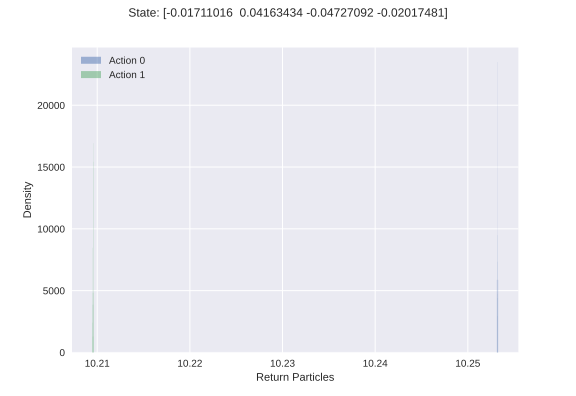
\includegraphics[scale=0.8]{results/ct51-cartpole-deterministic-returns}
  \caption[DEICIDE performance in a deterministic setting]{DEICIDE
    performance in \textsc{CartPole-v0}} 
  \label{fig:exp:cartpole:deterministic}
\end{figure}

We see that DEICIDE was able to accurately model the return
distributions as approximate Dirac measures.

\subsection{Deep DEICIDE}
Finally, we showcase the performance of DEICIDE in a continuous-time
stochastic setting. We modify the \textsc{CartPole-v0} benchmark
\citep{brockman2016openai} to create a benchmark, which we call
\textsc{NoisyContinousTimeCartPole-v0}, as follows:

\begin{itemize}
\item We sample timesteps $\tau\sim\mathsf{Exponential}(100) +
  10^{-3}$;
\item We perturb force inputs to the cart with Gaussian noise sampled
  from $\mathcal{N}(0, 1)$;
\item We provide three more actions to deal with noise: a ``NO-OP''
  action with applies no force, and a double force action in each direction.
\end{itemize}

We implement Algorithm \ref{alg:deicide:fd} with a deep neural network
estimating the $N=11$ quantile functions (and another for the target quantile
functions), as well as a deep neural network estimating the system
dynamics and trained via the reparameterization trick.

The experiment is run over several hyperparameter configurations and
random seeds, as suggested by \citet{henderson2018deep}. We see that
DEICIDE is fairly stable with respect to hyperparameter configurations
and seeds, as illustrated in Figure \ref{fig:exp:cartpole:stability}.

\begin{figure}[h]
  \centering
  \newcommand{\cartpolestabilityscale}[0]{0.34}
  \begin{minipage}{0.49\linewidth}
    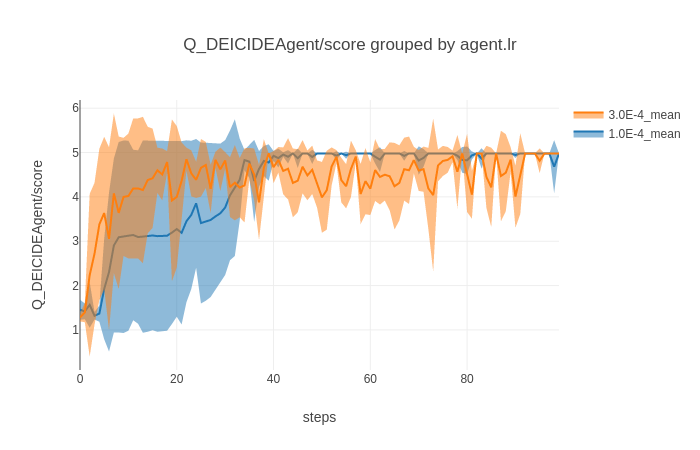
\includegraphics[scale=\cartpolestabilityscale]{results/ct-fd-cartpole-lr}
  \end{minipage}
  \begin{minipage}{0.49\linewidth}
    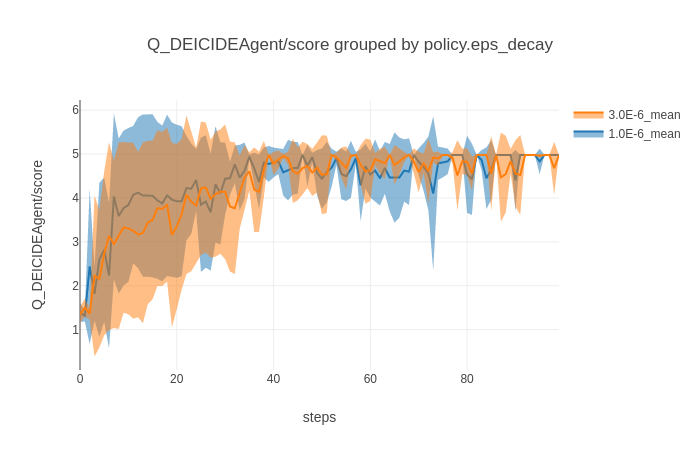
\includegraphics[scale=\cartpolestabilityscale]{results/ct-fd-cartpole-epsdecay}
  \end{minipage}
  \caption{Stability of DEICIDE with respect to hyperparameter
    configurations and random seeds}
  \label{fig:exp:cartpole:stability}
\end{figure}

Additionally, we see that the agents learned the optimal controller
very quickly. As an example, Figure
\ref{fig:exp:cartpole:returnmeasure} displays the return measure
function learned by the agent at a random initial state.

\begin{figure}[h]
  \centering
  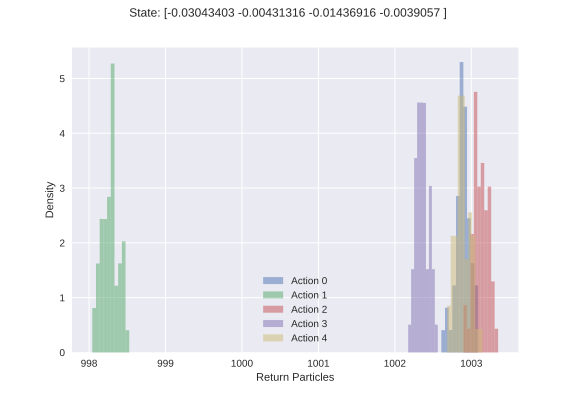
\includegraphics[scale=0.4]{results/ct51-fd-cartpole-returns}
  \caption{Return measure learned by a deep DEICIDE agent}
  \label{fig:exp:cartpole:returnmeasure}
\end{figure}
